\chapter{Einleitung}
\section{Motivation und Marktkontext}
Künstliche Intelligenz, Künstliche Intelligenz, Künstliche Intelligenz – kaum ein Thema dominiert die gegenwärtige technologische Landschaft so stark, wobei sich die drastischen Auswirkungen insbesondere auf dem Speichermarkt manifestieren. Die fundamentale Relevanz von High-Bandwidth DRAM für die Leistungsfähigkeit von Grafikprozessoren (GPUs) und spezialisierten Beschleunigern in KI-Rechenzentren führt zu einem immensen Nachfrage- und Profitabilitätsanstieg in diesem Segment. Infolgedessen werden Produktionskapazitäten systematisch von konventionellen Anwendungsbereichen abgezogen, was eine erhebliche Verknappung des Gesamtangebots und drastische Preissteigerungen – laut Counterpoint Research um 80 bis 90 Prozent im laufenden Quartal – zur Folge hat \cite{spectrum_dram_shortage}. Zur Begrenzung von Lieferkettenrisiken und zur Sicherung der technologischen Handlungsfähigkeit ist die Identifikation alternativer DRAM-Hersteller sowie eine herstellerunabhängige Auslegung des Leiterplattendesigns essenziell.

\section{Zielsetzung und Aufgabenstellung}
Aus diesem Hintergrund beschäftigt sich diese Arbeit mit der Simulation und Optimierung des FPGA–LPDDR4-Schnittstelle-Layouts zur Sicherstellung der Signalintegrität im Worst-Case-Betriebsbereich mit HyperLynx. Im Zentrum steht dabei ein herstellerübergreifender Ansatz: Anstatt das Layout auf die elektrischen Charakteristika eines einzelnen LPDDR4-Speicherbausteins auszulegen, ermöglicht die Simulation mit HyperLynx die gleichzeitige Berücksichtigung mehrerer Herstellerparameter. Durch die Integration von IBIS-Modellen unterschiedlicher Produzenten in eine gemeinsame Simulationsumgebung kann ein universell kompatibles Layout entwickelt werden, das Signalintegritätsanforderungen trotz unterschiedlichen Bauteilquelle erfüllt.

Um die methodische Vorgehensweise dieser Arbeit nachvollziehbar zu gestalten, werden im Folgenden die zentralen Fachbegriffe der These – FPGA, LPDDR4-Interface, Hyperlynx, Signalintegrität, Worst-Case-Betriebsbereich und PCB Layout – detailliert erläutert, um die technische Grundlage der durchgeführten Untersuchungen zu deklarieren.

\chapter{Theoretische und Technische Grundlagen}
\section{Architektonische Grundlagen des FPGA}
Ein FPGA (Field Programmable Gate Array) ist ein benutzerdefinierter Prozessor, dessen Hardware-Architektur nach der Fertigung frei konfigurierbar bleibt \cite{digilent_fpga}. Im Gegensatz zu fest verdrahteten Mikroprozessoren bestehen FPGAs aus einem Array programmierbarer Logikblöcke, die durch ein flexibles Routing-Netzwerk verbunden werden. Diese Struktur ermöglicht es Entwicklern, digitale Schaltungen maßgeschneidert auf spezifische Anwendungsanforderungen auszulegen – von einfachen Steuerlogiken bis hin zu komplexen Signalverarbeitungssystemen. Durch diese Flexibilität finden FPGAs breite Anwendung in Bereichen, wo hohe Rechenleistung bei gleichzeitig geringer Latenz gefordert ist.

\section{Funktionsweise und Merkmale von LPDDR4-Speichern}
Um die durch den FPGA verarbeiteten Daten zwischenzuspeichern und bei Bedarf schnell abrufen zu können, ist ein externer Arbeitsspeicher unerlässlich. Hier kommt LPDDR4 (Low Power Double Data Rate 4) zum Einsatz – ein energieeffizienter DRAM-Speichertyp, der speziell für mobile und platzbeschränkte Anwendungen entwickelt wurde. LPDDR4 überträgt Daten bei jeder Taktflanke (Double Data Rate), wodurch bei gleicher Taktfrequenz die doppelte Datenrate im Vergleich zu Single-Data-Rate-Speichern erreicht wird. Die Schnittstelle zwischen FPGA und LPDDR4 stellt somit eine kritische Verbindung dar, deren elektrische Eigenschaften maßgeblich die Systemleistung beeinflussen.

\section{Grundlagen der Signalintegrität (SI)}
Gegenstand der Simulation ist die Signalintegrität (SI – Signal Integrity), welche die Qualität elektrischer Signale während der Übertragung beschreibt. SI umfasst Aspekte wie Signalübersprechen (Crosstalk), Reflexionen an Impedanzsprüngen, Laufzeitverzögerungen sowie Rauscheinflüsse. Eine hohe Signalintegrität gewährleistet, dass digitale Signale ihren Zielbaustein unverfälscht erreichen und korrekt interpretiert werden. Bei Hochgeschwindigkeitsschnittstellen wie LPDDR4 mit Datenraten im Gigabit-Bereich können bereits minimale Layoutabweichungen zu Bitfehlern und Systeminstabilitäten führen. Auf die physikalischen Effekte sowie die konkreten Bewertungskriterien dieser Signalintegritätsaspekte wird im weiteren Verlauf dieses Berichts genauer eingegangen.

\section{Definition des Worst-Case-Betriebsbereichs}
Der Worst-Case-Betriebsbereich definiert die extremsten zulässigen Bedingungen, unter denen ein System noch fehlerfrei funktionieren muss. Dies ist dabei vom JEDEC-Standard definiert \cite{siemens_ddr_sim}. Die Taktfrequenz ist dabei frei wählbar, wobei die Signalintegritäts-Margins mit steigender Frequenz typischerweise abnehmen. Daher wird das Layout zunächst auf der maximal möglichen Frequenz ausgelegt, um ausreichende Reserven zu schaffen.
Als Obergrenze dient die niedrigere der beiden maximalen Frequenzen aus den Datenblättern: Während der LPDDR4-Speicher von Alliance Memory eine maximale Clock-Frequenz von 3200 Mbps (1600 MHz) unterstützt \cite{alliance_lpddr4_ds}, limitiert der Zynq UltraScale+ Memory Controller auf 2400 Mbps (1200 MHz, Speed Grade -1) \cite{xilinx_zynq_ds}. Somit wird das Design bei 2400 Mbps optimiert und abschließend bei der tatsächlichen Betriebsfrequenz validiert, um sicherzustellen, dass alle Signalintegritäts-Kriterien auch unter realen Bedingungen eingehalten werden.

\section{Softwaregestützte Analyse mittels HyperLynx}
Um die Zuverlässigkeit dieser Schnittstelle sicherzustellen, wird mittels virtueller Modelle in HyperLynx eine Simulation durchgeführt. HyperLynx von Siemens ist eine etablierte Softwarelösung zur Signal- und Power-Integrity-Analyse, die es ermöglicht, PCB-Layouts bereits in der Entwurfsphase auf potenzielle Probleme zu untersuchen. Durch die Integration von IBIS-Modellen (\textit{Input/Output Buffer Information Specification}) verschiedener Speicherhersteller können elektrische Charakteristika wie Impedanz, Laufzeiten und Reflexionen präzise berechnet werden, ohne physische Prototypen fertigen zu müssen. Auf die technischen Details dieser IBIS-Modelle sowie auf die detaillierten Simulationsparameter wird im weiteren Verlauf dieses Berichts genauer eingegangen. Dieser simulationsgestützte Ansatz reduziert Entwicklungszeit und Kosten erheblich.

\section{PCB-Layout und Design-Workflow in Mentor Xpedition}
Das in dieser Arbeit untersuchte Leiterplatten Design wurde mit der CAD-Software Mentor Xpedition von Siemens erstellt. Mentor Xpedition ist eine etablierte Lösung für komplexe PCB-Entwürfe und bietet umfassende Funktionen für Stackup-Definition, Routing und Design-Rule-Checking (DRC). Das Layout umfasst die Platzierung des Zynq UltraScale+ FPGA, der LPDDR4-Speicherbausteine sowie aller passiven und aktiven Komponenten. Eine detaillierte Darstellung des vollständigen PCB-Layouts mit allen relevanten Signalpfaden befindet sich in Anhang A (siehe Abbildung A.1).

Das zuvor beschriebene PCB-Layout bildet die physische Grundlage für die elektrische Verbindung zwischen FPGA und LPDDR4-Speicher. Um die Anforderungen an dieses Layout nachvollziehbar zu gestalten, werden im folgenden Kapitel die technischen Grundlagen der FPGA-LPDDR4-Schnittstelle erläutert. Diese umfassen die wesentlichen Signalgruppen sowie die Kriterien zur Bewertung der Signalqualität.

\chapter{Architektur und Signalgruppen der FPGA–LPDDR4-Schnittstelle}
Die Schnittstelle zwischen FPGA und LPDDR4-Speicher besteht aus mehreren koordinierten Signalgruppen, die gemeinsam einen zuverlässigen Datentransfer gewährleisten. Im Überblick umfasst das System die Taktleitung (Clock), die Daten-Strobe-Signale, die Adress- und Befehlsleitungen (Address/Command) sowie die Bewertungskriterien zur Signalintegrität in Form von Eye-Mask-Diagrammen. Jede dieser Komponenten erfüllt eine spezifische Funktion im Datenübertragungsprozess und unterliegt eigenen elektrischen Anforderungen. Für ein besseres Verständnis, wo diese Leitungen im Layout verbunden sind, betrachte dafür Abbildung \ref{fig:dram_ballout}.

\begin{figure}[ht]
    \centering
    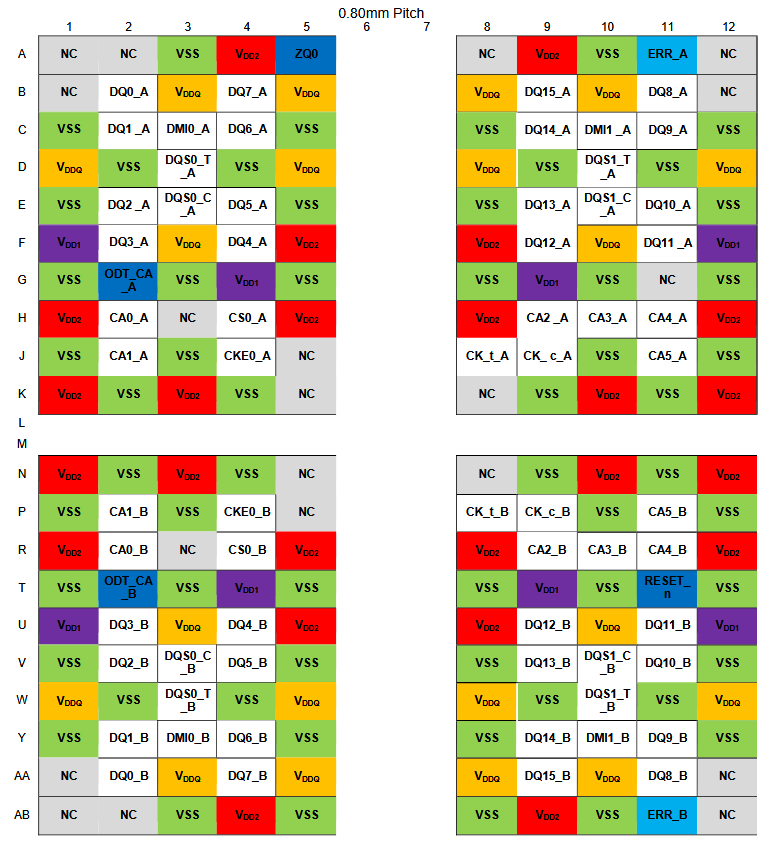
\includegraphics[width=\linewidth]{figures/DRAM-Ballout.png}
    \caption{Ballout eines LPDDR4 von Alliance Memory mit beschrifteten Takt-, Daten-, Strobe-, Adress- und Maskenleitungen.}
    \label{fig:dram_ballout}
\end{figure}

Im Folgenden werden nun diese Leitungen genauer erklärt.

\section{Taktübertragung (Clock-Signale)}
Das Clock-Signal ist das zentrale Synchronisationssignal der Schnittstelle. LPDDR4 verwendet einen differenziellen Takt (CK\_t und CK\_c), der sowohl steigende als auch fallende Flanken zur Datenübertragung nutzt (Double Data Rate). Der Takt referenziert alle Command-, Address- und Write-Operationen. Eine minimale Taktjitter-Toleranz ist entscheidend, da Timing-Abweichungen direkt die verfügbaren Setup- und Hold-Zeiten der Datenleitungen beeinflussen. Eine detaillierte Betrachtung dieser Setup- und Hold-Zeiten erfolgt in Abschnitt \ref{sec:timing_analyse}.

\section{Phasenbeziehungen der Daten-Strobe-Signale (DQS)}
Die differenziellen Daten-Strobe-Signale ($DQS\_t$ / $DQS\_c$) stellen die zeitliche Phasenreferenz für das Abtasten der Datenleitungen ($DQ$) bereit. Zur Gewährleistung maximaler Timing-Margen unterscheidet sich die Phasenbeziehung zwischen $DQS$ und $DQ$ je nach Zugriffsrichtung grundlegend (siehe Abbildung \ref{fig:read_write}):

\begin{itemize}
    \item \textbf{Lesezugriff (\textit{Read}):} Der Speicherbaustein treibt das $DQS$-Signal flankenbündig (\textit{edge-aligned}) zu den Daten. Die Signalflanken von $DQS$ fallen exakt mit den Zustandswechseln der $DQ$-Leitungen zusammen. Die empfängerseitige Logik (z. B. im FPGA) verschiebt $DQS$ intern über eine \textit{Delay-Locked Loop} (DLL) um 90°, um die Daten mittig im Datenauge abzutasten.
    \item \textbf{Schreibzugriff (\textit{Write}):} Der Treiber (FPGA) gibt das $DQS$-Signal bereits um 90° phasenverschoben (\textit{center-aligned}) bezüglich der $DQ$-Daten aus. Die Flanken von $DQS$ treffen zentriert im gültigen Datenfenster beim Speicher ein, was die Setup- und Hold-Zeiten maximiert.
\end{itemize}

Abbildung \ref{fig:read_write} veranschaulicht das Phasenverhältnis zwischen DQ und DQS im Lese- und Schreibzugriff.

\begin{figure}[ht]
    \centering
    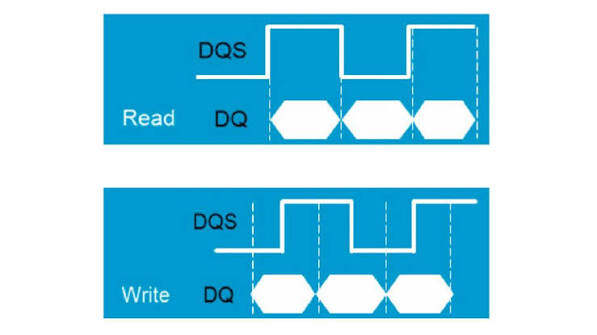
\includegraphics[width=\linewidth]{figures/read-write.jpg}
    \caption{Phasenbeziehung zwischen DQ und DQS bei Lese- und Schreibzugriff.}
    \label{fig:read_write}
\end{figure}

\section{Multiplexing im Command- und Adressbus (CA)}
Die Command- und Adressleitungen übertragen die Befehls- und Adressinformationen vom Controller zum Speicherbaustein. Um Stiftzahl und Platzbedarf zu reduzieren, wird bei LPDDR4 ein gemultiplextes Bus-Konzept eingesetzt, bei dem Befehle und Adressen über dieselben Leitungen zeitversetzt übertragen werden.

\section{Selektive Datensteuerung über die Schreibmaske (Write Mask)}
Bei der LPDDR4-Schnittstelle werden Daten parallel als Block übertragen – typischerweise 16 Byte pro Schreibzugriff bei einer x32-Organisation. Um jedoch kleinere Dateneinheiten innerhalb dieses Blocks adressieren zu können, wird zusätzlich eine Write Mask (DM-Signal) übertragen. Diese Maske gibt für jedes Byte im Datenblock an, ob es tatsächlich in den Speicher geschrieben werden soll oder nicht. Beispielsweise kann durch Setzen der entsprechenden Mask-Bits nur das erste Byte aktualisiert werden, während die restlichen 15 Byte des Blocks unverändert bleiben. Diese Funktionalität ermöglicht effiziente Teilzugriffe auf den Speicher, ohne dass gesamte Blöcke ausgelesen, modifiziert und zurückgeschrieben werden müssen \cite{lpddr_notes}.

\section{Qualitätsbewertung mittels Eye-Mask-Diagrammen}
Das Eye-Mask-Diagramm ist ein zentrales Bewertungswerkzeug zur Quantifizierung der Signalintegrität bei Hochgeschwindigkeitsschnittstellen. Es entsteht durch die Überlagerung vieler Bitperioden eines Signals in einem Oszilloskop oder einer Simulation. Die resultierende „Augenöffnung" visualisiert die verfügbare Spannungs- und Timing-Marge für eine fehlerfreie Signalabtastung.

\begin{figure}[ht]
    \centering
    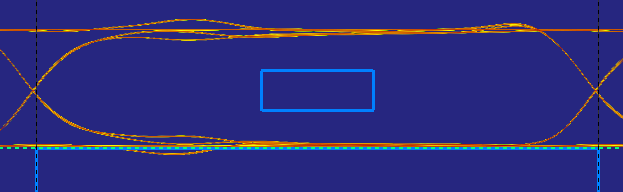
\includegraphics[width=\linewidth]{figures/eyemask.png}
    \caption{Hyperlynx Eye Diagramm für Datenleitungen mit nicht zulässigem Bereich als Augenmaske gekennzeichnet.}
    \label{fig:eyemask}
\end{figure}

Die \textbf{Eye-Mask} definiert einen verbotenen Bereich innerhalb des Augendiagramms, den das Signal nicht durchdringen darf. Diese Maske wird typischerweise aus den Spezifikationen des Speicherstandards (JEDEC) oder den Anforderungen des FPGA-Herstellers abgeleitet. Ein Signal, das die Eye-Mask verletzt, weist unzureichende Margen auf und kann zu Bitfehlern führen. In HyperLynx wird die Eye-Mask-Analyse verwendet, um die Margins für den Entwickler zu veranschaulichen (siehe Abbildung \ref{fig:eyemask}).

\chapter{Konfiguration und Durchführung der HyperLynx DDR-Simulation}
In Siemens HyperLynx (LineSim und BoardSim) steht ein breites Spektrum an Grundfunktionen zur Analyse der Signalintegrität (SI) zur Verfügung. Nach der Konstruktion und Extraktion von Übertragungsstrecken lassen sich die Signaleigenschaften über das integrierte virtuelle Oszilloskop detailliert untersuchen. Dazu gehören die Generierung von Augendiagrammen (Eye Diagrams), die Erfassung von Übersprechen (Crosstalk) sowie die Ermittlung transienter Signalantworten. Darüber hinaus erlaubt die Software die Modellierung differenzieller Signalpaare und das Überlagern mehrerer Simulationsergebnisse in der Oszilloskop-Darstellung. Dadurch können unterschiedliche Leitungsabschlüsse (Terminations) manuell konstruiert und direkt miteinander vergleichend analysiert werden.

Für umfassende Post-Layout-Simulationsabläufe ermöglicht die Schnittstelle zu Mentor (Siemens) Xpedition Layout den Export des vollständigen PCB-Layouts und dessen anschließenden Import in BoardSim. Dabei werden alle relevanten Leiterbahnparameter – wie Breiten, Längen sowie komplexe Kopplungseffekte – automatisch generiert und aus den Layoutdaten extrahiert.

\begin{figure}[ht]
    \centering
    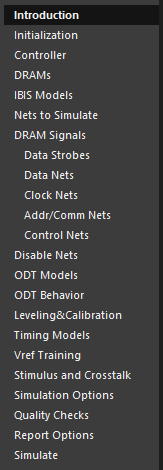
\includegraphics[width=\linewidth]{figures/config.png}
    \caption{Reiter für die Konfiguration des Hyperlynx DDRx-Wizards.}
    \label{fig:config}
\end{figure}

Abbildung \ref{fig:config} gibt einen Überblick über die wesentlichen Reiter und Einstellungsmenüs, die für die Durchführung einer automatisierten DDR4-Simulation konfiguriert werden müssen. Die folgenden Abschnitte konzentrieren sich auf spezifische Konfigurationseigenschaften des DDRX Batch Wizards.

\section{Integration und Relevanz herstellerspezifischer IBIS-Modelle}
Das \textbf{IBIS-Format (\textit{Input/Output Buffer Information Specification})} stellt ein standardisiertes Modell zur Beschreibung des elektrischen Verhaltens von Ein-/Ausgangspuffern integrierter Schaltungen dar \cite{ibis_faq}. Eine IBIS-Datei enthält dabei keine proprietären Schaltungsinformationen, sondern beschreibt das nichtlineare Verhalten der Puffer durch Spannungs-Strom-Kennlinien (V-I-Kurven), Schaltzeiten sowie Kapazitätswerte für verschiedene Prozess-, Temperatur- und Spannungsecken (Corners). Diese Informationen sind für eine präzise Simulation der Signalintegrität auf Leiterplattenebene essenziell.

IBIS-Modelle werden direkt von den Halbleiterherstellern bereitgestellt und müssen für die jeweiligen DRAM- und FPGA-Komponenten bei den Herstellern angefordert oder von deren Support-Portalen heruntergeladen werden. Im Rahmen dieser Arbeit wurden IBIS-Modelle der folgenden Hersteller beschafft und in die Simulation integriert:
\begin{itemize}
    \item \textbf{Xilinx Zynq} (FPGA/SoC-Plattform)
    \item \textbf{Integrated Silicon Solution Inc. (ISSI)} (DRAM-Hersteller)
    \item \textbf{Intelligent Memory} (DRAM-Hersteller)
\end{itemize}

Zur Validierung und Vergleichbarkeit der Simulationsergebnisse wurden zusätzlich IBIS-Daten von \textbf{Alliance Memory} herangezogen und die Simulationsergebnisse gegenübergestellt. Dieser herstellerübergreifende Ansatz gewährleistet eine Optimierung des Layouts. Dadurch wird die Auslegung des Layouts für mehrere Hersteller möglich.

\section{Dynamische Signalabschluss-Steuerung (On-Die Termination – ODT)}
Die On-Die Termination (ODT) ist ein integriertes Abschlussnetzwerk innerhalb der DDR-Speicherbausteine selbst. Im Gegensatz zu externen Abschlusswiderständen auf der Leiterplatte kann ODT dynamisch während des Betriebs aktiviert oder deaktiviert werden, was insbesondere bei hohen Datenraten von Vorteil ist. Durch die Integration des Abschlusses direkt im Chip werden Reflexionen an der Last minimiert und die Signalqualität verbessert. In HyperLynx muss der ODT-Wert entsprechend dem Speichertyp und der Betriebsfrequenz konfiguriert werden, um realistische Simulationsbedingungen abzubilden.

\section{Skew-Kompensation und Kalibrierung im zweistufigen Simulationslauf („Second Run“)}
Durch die Aktivierung der Option „Automatically run simulation 2 times“ (Second Run) im HyperLynx DDRx-Batch-Wizard wird eine zweistufige Simulationsdurchführung gewählt. Im ersten Durchlauf werden Laufzeitunterschiede (Skews) zwischen den Takt- und Datensignalen, die durch die typische Fly-By-Topologie entstehen, zunächst ermittelt und geschätzt. Im anschließenden zweiten Durchlauf („Second Run“) werden diese berechneten Skew-Werte unter Berücksichtigung der im Controller definierten Kalibrierungsoptionen – wie dem Write Leveling oder spezifischen DQS/DQ-Anpassungen – direkt angewendet \cite{xilinx_ultrascale_sim}. Dies ermöglicht eine deutlich präzisere Abbildung des realen Systemverhaltens inklusive der Controller-Kalibrierung.

\section{Betrachtung von Prozess-, Temperatur- und Spannungsschwankungen (PVT-Corners)}
Die Einstellung „IC Model with Typical Corners" definiert, welche Prozess-Temperatur-Spannungs-Ecken (PVT-Corners) für die Simulation verwendet werden. IBIS-Modelle enthalten typischerweise Daten für drei Ecken: \textbf{Minimum/Slow} (langsamster Prozess, niedrigste Temperatur, niedrigste Spannung), \textbf{Typical} (typische Betriebsbedingungen) und \textbf{Maximum/Fast} (schnellster Prozess, höchste Temperatur, höchste Spannung). Jede Ecke repräsentiert unterschiedliche Betriebszustände der Halbleiterkomponenten und ermöglicht somit die Bewertung des Systemverhaltens unter variierenden Bedingungen.

Im Rahmen dieser Arbeit wurde aufgrund des zeitlichen und umfangbedingten Rahmens ausschließlich mit den \textbf{Slow Corners} simuliert. Für eine umfassende Robustheitsprüfung im industriellen Kontext sollten jedoch zusätzlich die Typical- und Fast-Corners simuliert werden, um das Verhalten unter gesamten Betriebsbedingungen zu verifizieren.

\section{Berücksichtigung der JEDEC-Timing-Spezifikationen}

\chapter{Ergebnisse, Analyse und Layout-Optimierung}
\section{Gesamtauswertung der Simulationsergebnisse im DDRx Batch Wizard}
Nachdem alle zuvor beschriebenen Einstellungen im DDRx-Wizard konfiguriert und verifiziert wurden, konnte die eigentliche DDR-Simulation durchgeführt werden. Die nachfolgenden Abbildungen dokumentieren den Simulationsverlauf und die resultierenden Auswertungen, welche die Signalintegrität der LPDDR4-Schnittstelle bewerten.

Abbildung \ref{fig:summary} zeigt die Zusammenfassungsansicht (Summary) des HyperLynx DDRx-Batch-Wizards nach erfolgreich abgeschlossener Simulation. Die durchgängig grüne Kennzeichnung aller getesteten Parameter signalisiert, dass sämtliche Signalintegritäts-Anforderungen innerhalb der spezifizierten JEDEC-Toleranzen erfüllt werden. Um dieses Ergebnis zu erreichen, war insbesondere eine gezielte Anpassung des Leiterplattenlayouts hinsichtlich der Leiterbahnlängen erforderlich, da diese direkt die Setup- und Hold-Zeiten beeinflussen.

\begin{figure}[ht]
    \centering
    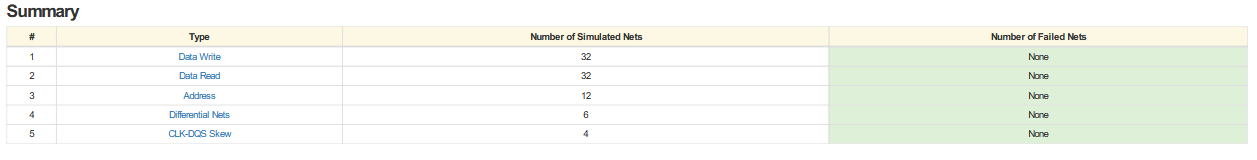
\includegraphics[width=\linewidth]{summary.png}
    \caption{Fehlerfreie Hyperlynx Simulation.}
    \label{fig:summary}
\end{figure}

\section{Timing-Analyse: Setup- und Hold-Zeiten}
\label{sec:timing_analyse}
Die \textbf{Setup-Time} definiert die minimale Zeitspanne, in der ein Datensignal vor der aktiven Strobe-Flanke stabil anliegen muss, damit der Speichercontroller die Daten korrekt erfassen kann. Abbildung \ref{fig:setup} veranschaulicht dies anhand einer Oszilloskop-Darstellung, bei der die Datenleitung vor der Strobe-Flanke ankommt und die erforderliche Setup-Marge eingehalten wird.

\begin{figure}[ht]
    \centering
    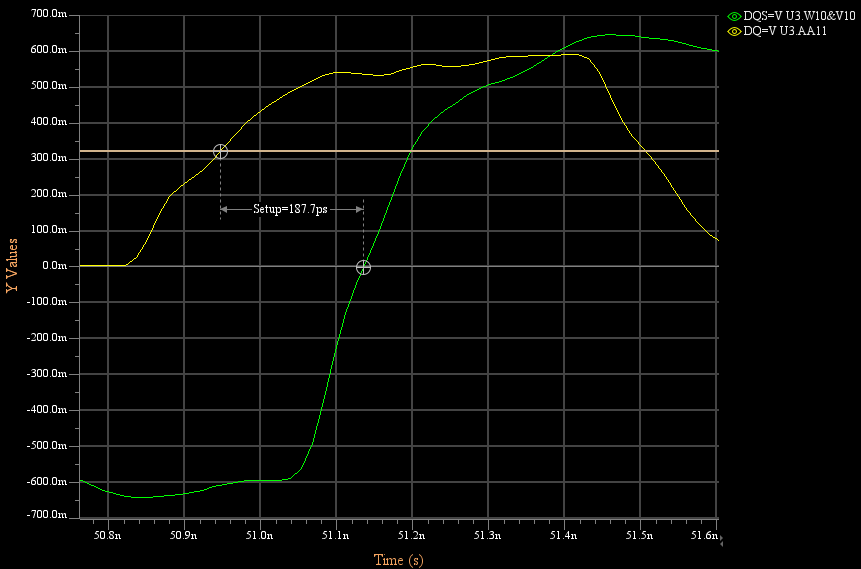
\includegraphics[width=\linewidth]{setup.png}
    \caption{Setup Time Darstellung in Hyperlynx.}
    \label{fig:setup}
\end{figure}

Die \textbf{Hold-Time} beschreibt hingegen die erforderliche Stabilitätsdauer des Datensignals nach der aktiven Strobe-Flanke, während der die Daten noch vom Speicherbaustein ausgelesen werden. Wie in Abbildung \ref{fig:hold} dargestellt, bleibt das Datensignal auch nach dem Auslesevorgang für die spezifizierte Hold-Zeit stabil erhalten, wodurch ein sicheres Sampling gewährleistet wird.

\begin{figure}[ht]
    \centering
    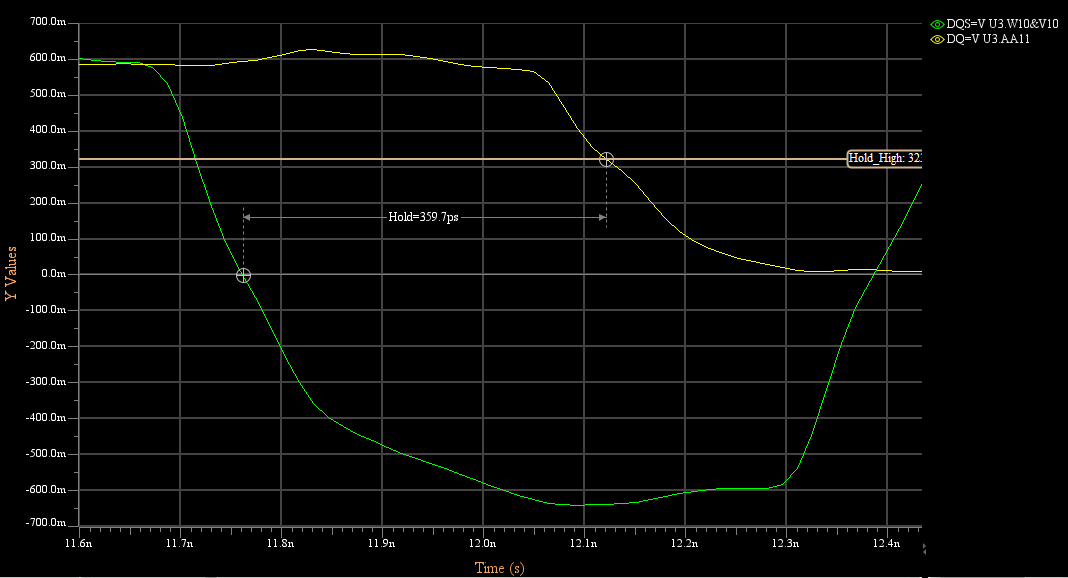
\includegraphics[width=\linewidth]{hold.png}
    \caption{Hold Time Darstellung in Hyperlynx.}
    \label{fig:hold}
\end{figure}

Setup- und Hold-Zeit stehen in einem direkten Verhältnis zueinander, wobei das Timing-Optimum bei symmetrisch ausgeglichenen Margen liegt, die den jeweiligen Standard übertreffen. Weicht dieses Verhältnis vom Ideal ab, müssen die Leiterbahnen entsprechend angepasst werden. Ist die Hold-Margin zu groß und die Setup-Zeit zu klein, muss das Signal früher am Empfänger ankommen, weshalb die Leitung verkürzt werden muss. Ist die Hold-Margin hingegen zu klein und die Setup-Zeit zu groß, verhält es sich umgekehrt, wodurch eine Verlängerung der Leitung erforderlich wird, um eine robuste Signalintegrität sicherzustellen.

\section{Einfluss von High-Speed-Layout-Richtlinien auf die Signalqualität}
Das erfolgreiche Abschneiden der Simulation ist maßgeblich darauf zurückzuführen, dass bereits während des Layout-Designs wesentliche High-Speed-Design-Richtlinien konsequent umgesetzt wurden. Ein entscheidender Faktor war die Führung der DDR-Datenleitungen ausschließlich auf inneren Lagen der Leiterplatte, wobei diese Signallagen beidseitig von Masseflächen (GND-Planes) eingeschlossen sind. Diese Abschirmung gewährleistet eine kontrollierte Impedanz, minimiert externe Störeinflüsse und reduziert die elektromagnetische Abstrahlung erheblich. Zudem wurde bei der Leiterbahnführung die sogenannte „3W-Regel" angewendet, bei der der Abstand zwischen benachbarten Signalleitungen ungefähr das Dreifache der Leiterbahnbreite beträgt. Diese etablierte Daumenregel reduziert kapazitive und induktive Kopplungseffekte (Crosstalk) zwischen parallelen Leitungen signifikant und trägt somit direkt zur Einhaltung der Signalintegritätsanforderungen bei \cite{nxp_lpddr4_guidelines}. Die Kombination aus geschirmter Layer-Stackup-Architektur und ausreichendem Leiterbahnabstand schuf somit die physikalische Grundlage für die positiven Simulationsergebnisse, da kritische Störmechanismen bereits im Layout minimiert wurden.

\section{Herstellerübergreifende Kompatibilitätsverifikation}
Um eine herstellerübergreifende Kompatibilität der LPDDR4-Schnittstelle zu gewährleisten, wurden die Datenleitungen auf die Einhaltung der Setup- und Hold-Zeiten im Worst-Case-Betriebsbereich bei 2400 MHz optimiert. Anschließend erfolgte eine Verifikation der Simulationsergebnisse mit IBIS-Modellen dreier verschiedener DRAM-Hersteller, namentlich Alliance Memory (AM), Integrated Silicon Solution Inc. (ISSI) und Intelligent Memory (IM) (siehe Anhang). Die Simulationsergebnisse belegen, dass das entwickelte Layout mit den gewählten Simulationsoptionen herstellerunabhängig sämtliche JEDEC-Spezifikationen erfüllt. Die detaillierten Auswertungen für alle drei Hersteller sind im Anhang dokumentiert (siehe Anhang A.X bis A.Z). Dies ermöglicht einen flexiblen Bauteilewechsel im Produktionsprozess ohne layouttechnische Modifikationen.

\chapter{Fazit und Ausblick}
Die im Rahmen dieser Arbeit durchgeführten HyperLynx DDR-Simulationen konnten erfolgreich abgeschlossen werden und bestätigen die Signalintegrität der entworfenen LPDDR4-Schnittstelle. Für eine weiterführende und noch umfassendere Validierung wären jedoch zusätzliche Simulationen wünschenswert. Dazu gehören unter anderem Mask-Simulationen zur detaillierteren Bewertung der Signalqualität, vertiefte Crosstalk-Analysen zur Quantifizierung von Nebensprechen zwischen benachbarten Leitungen sowie Simulationen mit Strong Corners zur Abbildung weiterer Prozessvariationen. Zudem war eine Integration der offiziellen Xilinx-Timing-Files für den Zynq-Controller vorgesehen, um die Simulation noch näher an die realen Controller-Eigenschaften anzupassen. Diese Erweiterungen konnten im Rahmen dieser Projektarbeit leider nicht mehr umgesetzt werden. Begründet liegt dies zum einen in der intensiven Einarbeitungszeit in das komplexe HyperLynx-Simulationswerkzeug und den zeitlichen Aufwand für die Beschaffung der IBIS-Modelle von den verschiedenen Herstellern. Zum anderen hat sich der Xilinx-Support trotz mehrfacher Kontaktversuche nicht bezüglich der angeforderten Timing-Files zurückgemeldet, wodurch diese Daten nicht in die Simulation einfließen konnten.